In this section we demonstrate the methods described so far and implemented in the software using a simple scenario. The network, shown in Figure \ref{fig:config}, has six links numbered 0 through 5. Links 0 through 4 have flow capacities of 2,000 veh/hour, while link 5 has a capacity of 1,00 veh/hour. All links except for link 2 are 200 meters in length. Link 2 is 400 meters. The free-flow speed in all links is 70 km/hr, and hence the free-flow travel time for all links except link 2 is about 10 seconds, while for link 2 it is about 20 seconds. There are two origin/destination pairs: OD 1, going from source node 0 to sink node 5, and OD 2, going from source node 1 to sink node 5. There are two paths available to OD 1: path 1, consisting of links [0, 3, 4, 5], and path 2 consisting of links [0, 2, 4, 5]. OD 2 is confined to path 3 = [1, 3, 4, 5]. Path [1, 2, 4, 5] is not utilized.

This network was chosen because it is small enough that the results are intuitive, and yet it illustrates the essential differences between the models and travel time functions described in Section~\ref{sec:models}. Only OD pair 1 (from 0 to 5) has a choice of route, and hence the assignment problem is only to decide how the demand for OD 1 is split between paths 1 and path 2, at each time interval. The total demand for both ODs will be set to a value that exceeds the capacity of link 5, and hence we expect congestion to form and propagate upstream past link 4, and onto to links 2 and 3, regardless of the assignment. Because path 1 is shorter than path 2, OD 1 should choose that path 1 until the accumulated congestion on link 3 causes its travel time to be as large or larger than that of link 2. Then the assignment should distribute traffic on paths 2 and 3 such that the travel times along paths 1 and 2 are equalized. 

\begin{figure}[h]
    \centering
    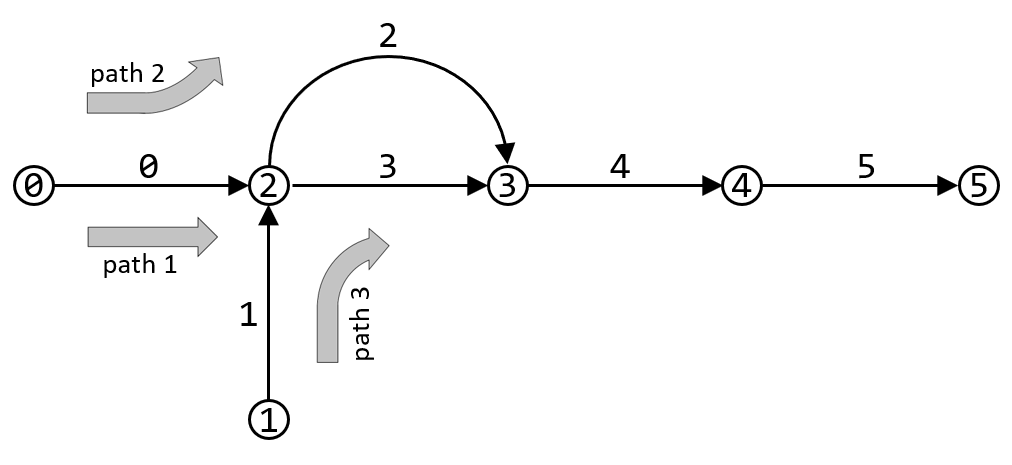
\includegraphics[width=\linewidth]{figs/config.png}
    \caption{Traffic network.}
    \label{fig:config}
\end{figure}

\subsection{Static assignment}
The static assignment problem is the simplest form of traffic assignment. It is posed with the static model and travel time functions of Eqs. (\ref{eq:staticmodel}) through (\ref{eq:bpr}), and solved with the Frank-Wolfe algorithm. Figure \XXX shows solutions to the problem with $\gamma$ ranging from 0 to 5. The plot shows that the demand assigned to path 1 is inversely proportional to $\gamma$. This fact can be easily ascertained by noting that the equilibrium condition requires the travel times on links 2 and 3 to be equal. 
\begin{equation}
\tau_2(h_2) = \tau_3(h_1 + h_3)
\end{equation}
Using Eq.(\ref{eq:bpr}) and with some manipulation we find,
\begin{equation}
asdf
\end{equation}
This formula is overlaid in Figure \XXX, demonstrating that the algorithm has indeed found the equilibrium solution in all cases. 
 
\subsection{Dynamic assignment}



Figure \XXX shows the equilibrium solution under the MN model. This solution was computed using the \XXX algorithm, and completed after \XXX iterations (~\XXX seconds)

DESCRIBE THE RESULT

Figure \XXX shows the equilibrium solution under the CTM model and both instantaneous and predictive travel time. This solution was computed using the \XXX algorithm, and completed after \XXX iterations (~\XXX seconds)

QUALITATIVE COMPARISON OF THE RESULTS.


\begin{figure}[h]
    \centering
    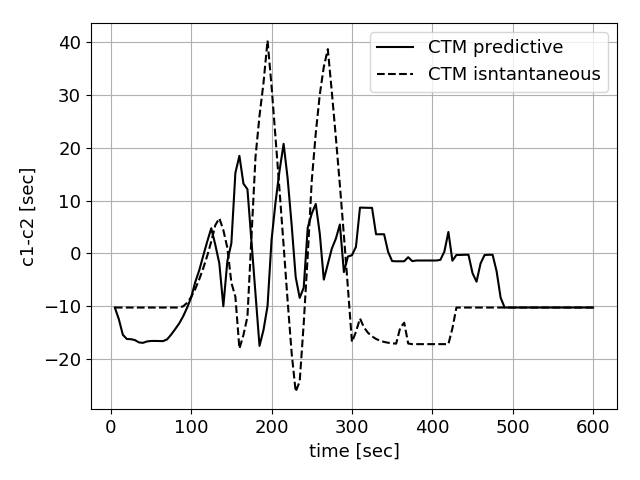
\includegraphics[width=0.9\linewidth]{figs/cdiff_1300.png}
    \caption{\XXX }
    \label{fig:cdiff}
\end{figure}

\begin{figure}[h]
    \centering
    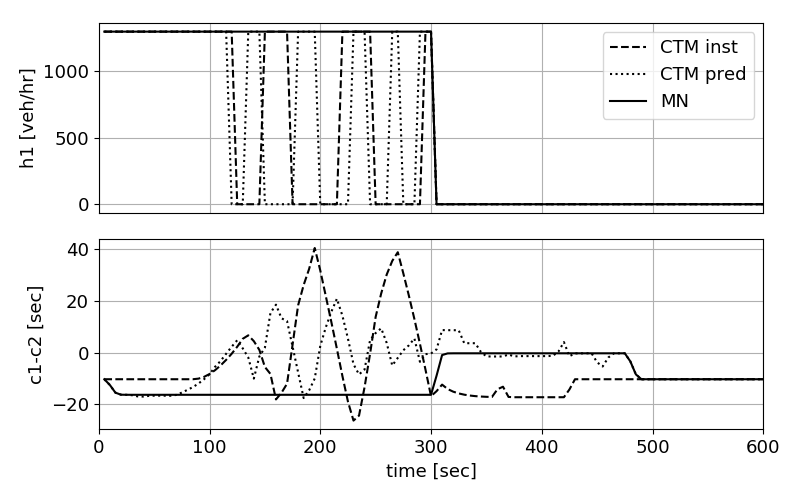
\includegraphics[width=\linewidth]{figs/ctm_vs_mn_hc.png}
    \caption{\XXX }
    \label{fig:ctm_vs_mn_hc}
\end{figure}

\begin{figure}[h]
    \centering
    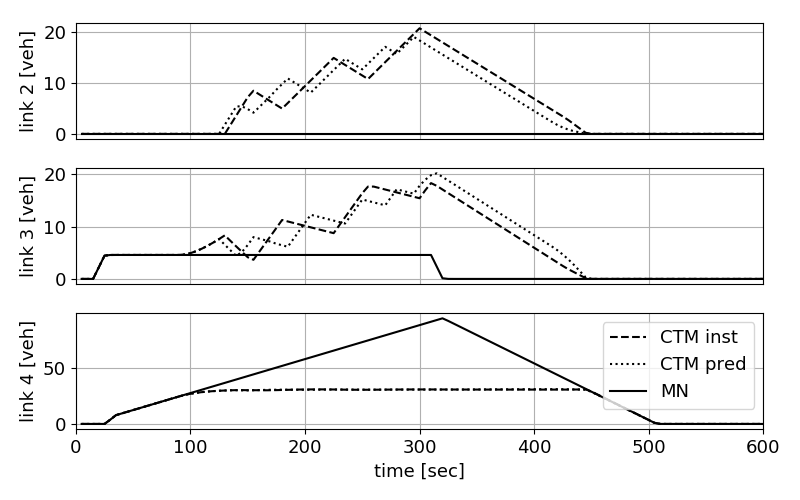
\includegraphics[width=\linewidth]{figs/ctm_vs_mn_x.png}
    \caption{\XXX }
    \label{fig:ctm_vs_mn_x}
\end{figure}

\begin{figure}[h]
    \centering
    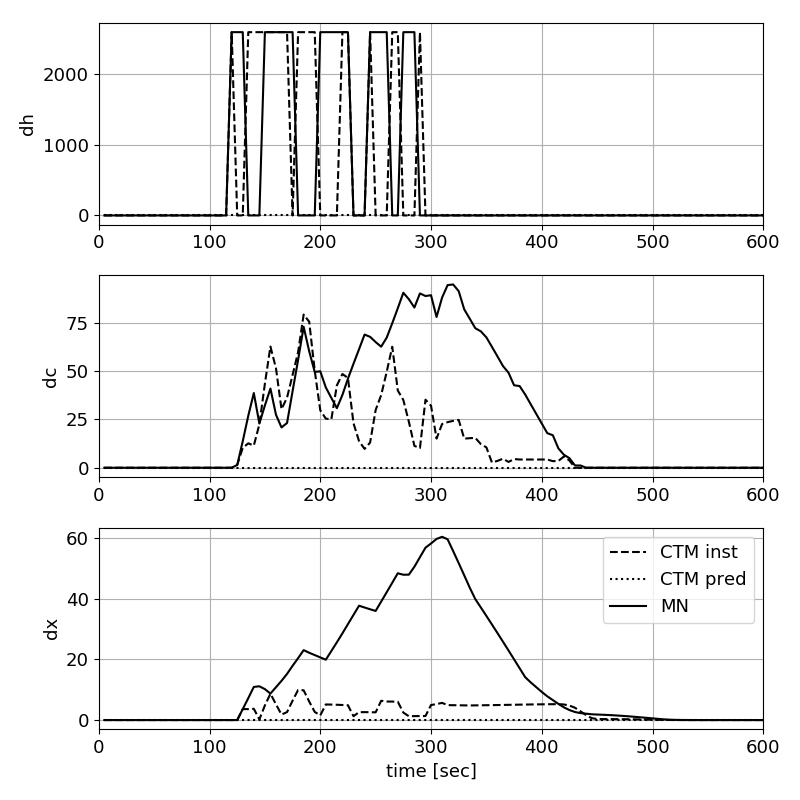
\includegraphics[width=\linewidth]{figs/dist2ctm.png}
    \caption{\XXX }
    \label{fig:dist2ctm}
\end{figure}

\begin{figure}[h]
    \centering
    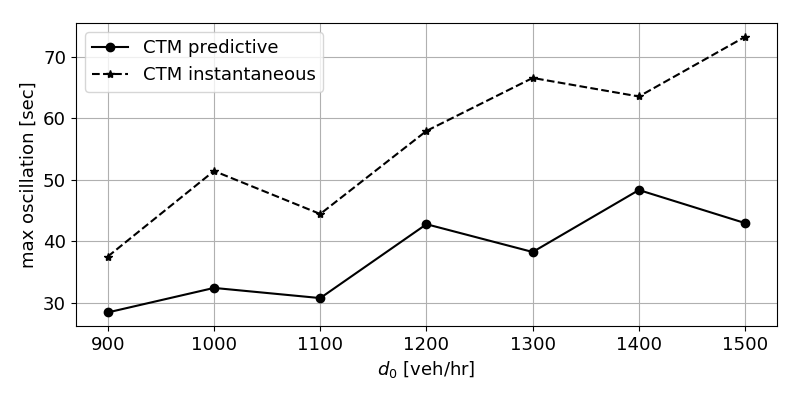
\includegraphics[width=\linewidth]{figs/peaks.png}
    \caption{\XXX }
    \label{fig:peaks}
\end{figure}

% \begin{figure}[h]
%     \centering
%     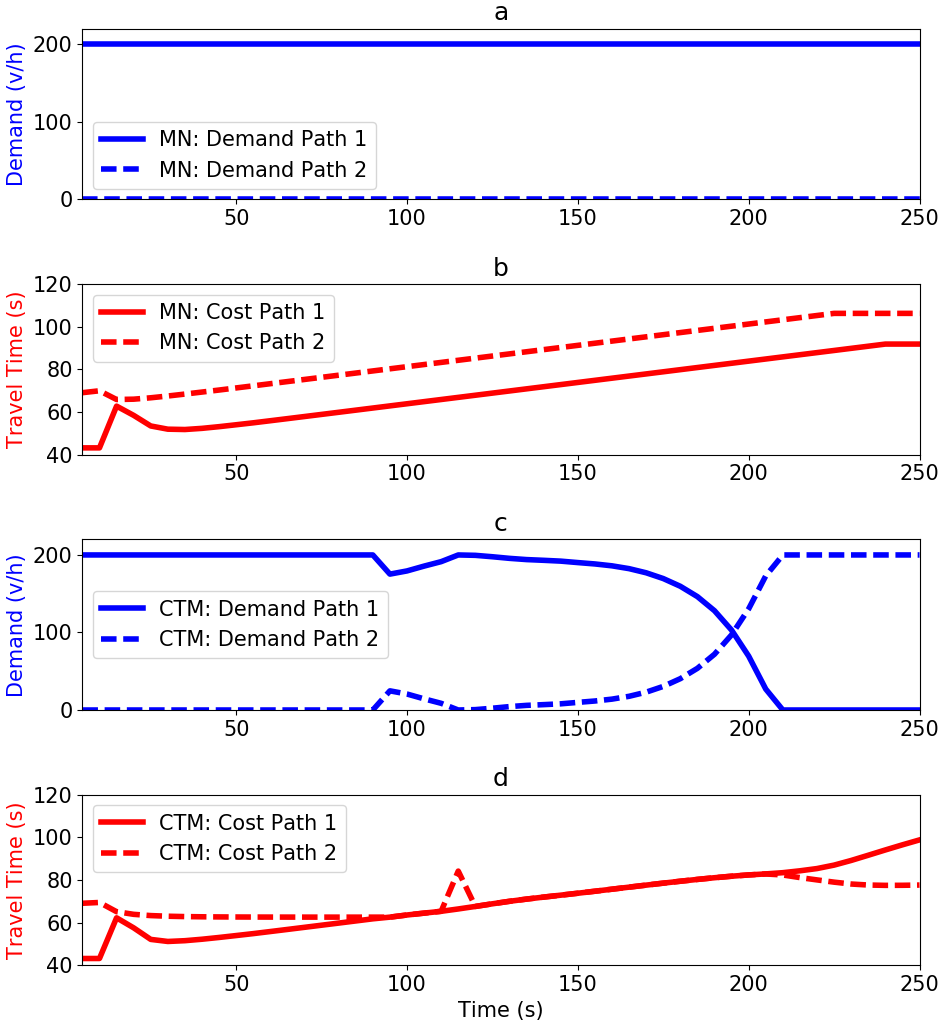
\includegraphics[width=\linewidth]{figs/Paper_dta_results_mn_ctm.PNG}
%     \caption{a. MN Equilibrium Assignment on Path 1 and 2 b. MN Travel Time on Path 1 and 2 c. CTM Equilibrium Assignment on Path 1 and 2 d. CTM Travel Time on Path 1 and 2 }
%     \label{fig:DTA_Results}
% \end{figure}

